\documentclass[tikz,border=6pt]{standalone}
\usepackage{amsmath,amssymb}
\usepackage{xcolor}
\definecolor{accent}{HTML}{A13D2C}
\definecolor{accent2}{HTML}{2B5F6B}
\definecolor{muted}{HTML}{5A564F}
\definecolor{panel}{HTML}{F8F6F0}
\definecolor{linecol}{HTML}{D8D2C4}
\definecolor{astroblue}{HTML}{1B4F72}
\definecolor{sunyellow}{HTML}{E8A33D}
\definecolor{colthree}{RGB}{60,140,80}
\usetikzlibrary{calc,arrows.meta,plotmarks}
\IfFileExists{results/ch12/lane_emden_n3.dat}{\def\datadir{results/ch12/}}{\def\datadir{../results/ch12/}}
\begin{document}
% Eddington standard model (n = 3 polytrope) scaled to the Sun: columns r/R, rho/rho_c, T/T_c, P/P_c, m/M.
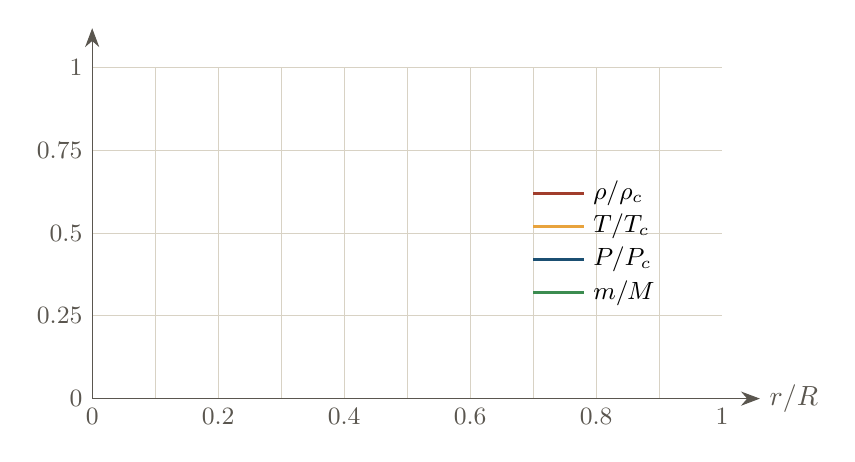
\begin{tikzpicture}[x=8cm,y=4.2cm, >={Stealth[length=2.4mm]}]
  \draw[linecol] (0,0) grid[xstep=0.1,ystep=0.25] (1,1);
  \draw[->, muted] (0,0) -- (1.06,0) node[right] {$r/R$};
  \draw[->, muted] (0,0) -- (0,1.12);
  \foreach \x in {0,0.2,0.4,0.6,0.8,1} \node[below, muted] at (\x,0) {\small \x};
  \foreach \y in {0,0.25,0.5,0.75,1} \node[left, muted] at (0,\y) {\small \y};
  \draw[accent, line width=1.1pt] plot file {\datadir sun_n3_rho.dat};
  \draw[sunyellow, line width=1.1pt] plot file {\datadir sun_n3_T.dat};
  \draw[astroblue, line width=1.1pt] plot file {\datadir sun_n3_P.dat};
  \draw[colthree, line width=1.1pt] plot file {\datadir sun_n3_m.dat};
  \foreach \c/\lab/\y in {accent/{$\rho/\rho_c$}/0.62, sunyellow/{$T/T_c$}/0.52, astroblue/{$P/P_c$}/0.42, colthree/{$m/M$}/0.32} {
    \draw[\c, line width=1.1pt] (0.70,\y) -- (0.78,\y); \node[right] at (0.78,\y) {\small \lab};
  }
\end{tikzpicture}
\end{document}
